\documentclass[10pt,a4paper]{article}

\usepackage[T1]{fontenc}
\usepackage{lmodern}
\usepackage[left=18mm,right=18mm,top=17mm,bottom=18mm,headheight=20pt,headsep=3mm]{geometry}
\usepackage{microtype}
\usepackage{xcolor}
\usepackage{graphicx}
\usepackage{amsmath,amssymb}
\usepackage{booktabs}
\usepackage{tabularx}
\usepackage{enumitem}
\usepackage{titlesec}
\usepackage{tcolorbox}
\usepackage{tikz}
\usetikzlibrary{arrows.meta,positioning,fit,calc}
\usepackage[colorlinks=true,linkcolor=black,urlcolor=blue!55!black]{hyperref}
\hypersetup{pdftitle={Towards a Minimal Autopoietic, Heritable Cell},pdfsubject={Compact design note for a 2D artificial chemistry}}
\usepackage{fancyhdr}

\definecolor{ink}{HTML}{17212B}
\definecolor{accent}{HTML}{0F6E75}
\definecolor{accent2}{HTML}{C95C35}
\definecolor{soft}{HTML}{EEF5F5}
\definecolor{soft2}{HTML}{FBF1EC}
\definecolor{muted}{HTML}{5D6872}
\definecolor{rulegray}{HTML}{D7DEE3}

\color{ink}
\setlength{\parindent}{0pt}
\setlength{\parskip}{4.5pt}
\setlist[itemize]{leftmargin=1.25em,itemsep=1.2pt,topsep=2pt}
\setlist[enumerate]{leftmargin=1.35em,itemsep=1.2pt,topsep=2pt}

\titleformat{\section}{\large\bfseries\color{accent}}{}{0pt}{}[\vspace{-2pt}\color{rulegray}\titlerule]
\titleformat{\subsection}{\normalsize\bfseries\color{ink}}{}{0pt}{}
\titlespacing*{\section}{0pt}{10pt}{5pt}
\titlespacing*{\subsection}{0pt}{7pt}{2pt}

\pagestyle{fancy}
\fancyhf{}
\fancyhead[L]{\small\color{muted}Minimal Autopoietic Cell - Design Note}
\fancyhead[R]{\small\color{muted}2D artificial chemistry}
\fancyfoot[C]{\small\color{muted}\thepage}
\renewcommand{\headrulewidth}{0.3pt}
\renewcommand{\headrule}{\hbox to\headwidth{\color{rulegray}\leaders\hrule height \headrulewidth\hfill}}

\newtcolorbox{principle}[1][]{
  colback=soft,colframe=accent!55!black,boxrule=0.6pt,arc=2mm,
  left=2.5mm,right=2.5mm,top=1.8mm,bottom=1.8mm,#1}
\newtcolorbox{warningbox}[1][]{
  colback=soft2,colframe=accent2!70!black,boxrule=0.6pt,arc=2mm,
  left=2.5mm,right=2.5mm,top=1.8mm,bottom=1.8mm,#1}

\newcommand{\code}[1]{\texttt{#1}}
\newcommand{\life}[1]{\textbf{\color{accent}#1}}

\begin{document}

\begin{center}
{\fontsize{22}{25}\selectfont\bfseries Towards a Minimal Autopoietic, Heritable Cell}\par
\vspace{2mm}
{\large\color{muted}A compact design note for a 2D artificial chemistry}\par
\vspace{3mm}
\begin{minipage}{0.92\textwidth}
\small
The objective is not to reproduce modern biology. It is to construct the simplest spatial universe in which a bounded object can maintain itself, repair damage, consume external resources, reproduce its internal organization, divide, inherit variable information, and let that information alter function. The central constraint is that the simulator should not contain a hidden ``cell program'': global biological behavior should arise from local mechanics, local bonding, diffusion, and bounded chemical rewrite rules.
\end{minipage}
\end{center}

\vspace{2mm}
\begin{principle}
\textbf{Design criterion.} We are allowed to make the artificial chemistry unusually favorable to life, but we should hard-code \emph{primitive physical opportunities}, not global goals. No rule should ask whether an object is a cell, whether a genome is complete, whether a copy has reached length six, or whether division ought to occur.
\end{principle}

\section{1. Target organism}

The intended organism is a deliberately small pseudo-cell: a deformable vesicle containing a population of short heritable polymers, functional polymers made from those sequences, and a small autocatalytic chemical network. It lives in a 2D bath supplying food or activated precursors.

\begin{center}
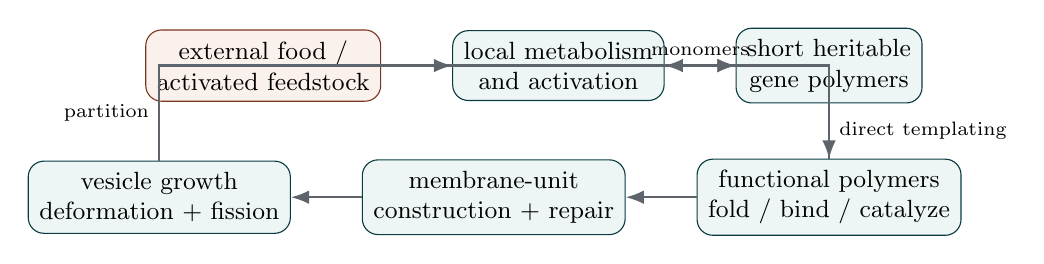
\begin{tikzpicture}[
  >=Latex, node distance=7mm and 9mm,
  box/.style={draw=accent!55!black, rounded corners=2mm, fill=soft, align=center, inner sep=4pt, font=\small},
  ext/.style={draw=accent2!60!black, rounded corners=2mm, fill=soft2, align=center, inner sep=4pt, font=\small},
  arr/.style={->, thick, draw=ink!70}
]
\node[ext] (food) {external food /\\activated feedstock};
\node[box, right=of food] (met) {local metabolism\\and activation};
\node[box, right=of met] (genes) {short heritable\\gene polymers};
\node[box, below=of genes] (func) {functional polymers\\fold / bind / catalyze};
\node[box, left=of func] (mem) {membrane-unit\\construction + repair};
\node[box, left=of mem] (ves) {vesicle growth\\deformation + fission};
\draw[arr] (food) -- (met);
\draw[arr] (met) -- node[above,font=\scriptsize]{monomers} (genes);
\draw[arr] (genes) -- node[right,font=\scriptsize]{direct templating} (func);
\draw[arr] (func) -- (mem);
\draw[arr] (mem) -- (ves);
\draw[arr] (ves) |- node[pos=0.25,left,font=\scriptsize]{partition} (genes);
\draw[arr] (func) |- (met);
\end{tikzpicture}
\end{center}

A successful run should eventually demonstrate the following life-like functions:

\begin{itemize}
\item \life{Integrity and homeostasis:} the compartment remains bounded while matter flows through it and internal concentrations fluctuate around viable ranges.
\item \life{Autopoiesis and repair:} membrane material is continuously rebuilt from internal chemistry; damage creates local opportunities for the same construction pathway to close the wound.
\item \life{Heredity:} information-bearing polymers copy themselves with finite fidelity and are physically partitioned at division.
\item \life{Programmable function:} sequence changes alter the construction or catalytic behavior of internal molecular machines without adding a new simulator-side particle type for every function.
\item \life{Reproduction:} membrane growth drives purely mechanical deformation and fission; daughter compartments then recover their internal steady state from inherited material.
\end{itemize}

\section{2. The artificial 2D universe}

The proposed universe has only a few primitive concepts. Particles have position, orientation, type, local interaction patches, and a bounded number of bonds. The spatial grid is only a contact finder. Chemistry is expressed as local graph rewrites involving a fixed number of nearby particles and directly bonded neighbors.

\begin{tabularx}{\textwidth}{@{}p{0.21\textwidth}X X@{}}
\toprule
\textbf{Primitive} & \textbf{Meaning} & \textbf{Constraint} \\
\midrule
Spatial motion & diffusion, excluded volume, short-range attraction / repulsion & no long-range recruitment toward a biological target \\
Saturable ports & directional bonds with finite valence & topology follows local compatibility, not global aggregate identity \\
Backbone bonds & stable polymer structure & strong relative to temporary template bonds \\
Pairing / docking bonds & reversible recognition between compatible sites & local, saturable, normally one partner per site \\
Reaction rules & bounded graph + geometry rewrites & inspect only a small neighborhood \\
Environmental phase & optional association / release cycle & global energy scaffold, not a cell-specific controller \\
\bottomrule
\end{tabularx}

\begin{principle}
\textbf{Locality test.} A rule is acceptable if it can be stated using a handful of particles, their direct bond neighbors, their free ports, and their relative geometry. The simulator may know the whole system for bookkeeping and statistics, but the reaction itself must not depend on global labels such as ``vesicle'', ``gene'', ``daughter'', or ``complete copy''.
\end{principle}

\section{3. Compartment: from patch particle to constructed membrane chemistry}

The current patch-particle vesicle demonstrator already provides a useful mechanical target: directional, saturable lateral bonds, a preferred turning angle, core repulsion, reversible rupture, and local rebinding generate flexible closed loops without assigning vesicle identifiers.

The next abstraction step is to stop treating the membrane unit as a magical single particle. A membrane-forming molecule should itself be a small aggregate assembled from generic modules, for example

\[
\text{membrane unit} \sim L - J - R \quad \text{with a polar / repulsive module } H \text{ attached to } J.
\]

Here $L$ and $R$ provide saturable lateral ports, $J$ fixes geometry, and $H$ gives the unit an oriented surface interaction. Different arrangements of the same small module alphabet can then change preferred curvature, adhesion, permeability, or robustness. A molecule is ``membrane-like'' because of what its exposed ports and geometry do, not because the engine calls it a lipid.

\subsection{Growth and repair}

Internal metabolism should preferably produce \emph{inactive membrane precursors}, not fully active membrane monomers. A free active monomer would tend to polymerize inside the vesicle and form useless fragments before reaching the shell. Instead, a precursor becomes incorporated only when a local membrane environment completes the reaction geometry.

A minimal local insertion rule is conceptually
\[
A{-}B + P_0 \longrightarrow A{-}P{-}B,
\]
where $A{-}B$ is an existing membrane bond and $P_0$ is a soluble precursor. In the more mature composite-molecule version, a membrane-bound catalyst assembles or activates the new membrane unit directly at an exposed or strained membrane site.

This provides repair almost for free. Damage produces unsaturated ports, strained edges, and locally exposed binding geometries. The same chemistry responsible for normal turnover and growth therefore has an increased probability of filling a hole. No explicit ``repair mode'' is required.

\section{4. Heritable polymers: role-free exact template copying}

The current template-copy demonstrator uses exact rather than complementary copying because biological complementarity is not required by the conceptual objective. A small alphabet is sufficient; binary is ideal for debugging, while a four-symbol alphabet gives a richer later sequence space.

Let $A$ and $B$ be backbone neighbors and let $a$ and $b$ be particles paired to them. The key ligation rule is symmetric:

\[
\begin{array}{ccc}
A & {-} & B\\[-1mm]
| & & |\\[-1mm]
a & & b
\end{array}
\quad \longrightarrow \quad
\begin{array}{ccc}
A & {-} & B\\[-1mm]
| & & |\\[-1mm]
a & {-} & b
\end{array}
\]

provided the lower ports are free and the four-particle geometry is compatible. There is no persistent \code{Template} or \code{Copy} role. Either bonded side can catalyze formation of the missing parallel backbone bond on the opposite side. The rule knows only a local quadrilateral.

Free monomers reach pairing range through diffusion. The simulator does not pull a correct monomer across the box. A local recognition patch favors same-symbol pairing; once paired, the matrix geometry aligns adjacent recruits so that backbone ligation becomes possible.

\subsection{Association and release}

There is a genuine physical tension between ``bind strongly enough to copy'' and ``separate after copying''. The simplest demonstrator uses an external periodic energy scaffold:

\begin{enumerate}
\item \textbf{Association / ligation phase:} reversible pairing is favorable and local templated backbone ligation can occur.
\item \textbf{Release phase:} pairing bonds become weak and thermal motion separates the polymers; backbone bonds remain strong.
\end{enumerate}

The phase change never checks copy length or sequence completeness. Partial products can detach; complete copies succeed only when kinetics happened to finish in time. Eventually this external cycle should be replaceable by chemically powered separation or helper molecules, but it is an acceptable first scaffold because it supplies energy rather than biological intent.

\section{5. Direct expression: sequence to functional polymer}

A central goal is to introduce an information-to-function indirection without reproducing DNA, RNA, ribosomes, and modern translation. The proposed shortcut is \emph{direct templated expression}.

Each gene symbol $G_i$ can participate in two chemically distinct matching interactions:

\[
G_i \leftrightarrow G_i \qquad \text{(exact genome copy)},
\]
\[
G_i \leftrightarrow F_i \qquad \text{(functional-polymer synthesis)}.
\]

The same local quadrilateral ligation rule can build either product. A gene such as
\[
G_0-G_2-G_1-G_3
\]
can therefore template both another $G_0-G_2-G_1-G_3$ chain and a physically different functional chain
\[
F_0-F_2-F_1-F_3.
\]

No reader scans the full gene and no table maps a complete sequence to a named protein. Chain ends can be represented by terminal chemistry or caps rather than a global length counter.

\subsection{How function should emerge}

The $F_i$ monomers should differ only in primitive physical properties: preferred backbone angle, local stiffness, hydrophobic / adhesive patch type, substrate affinity, or catalytic site. Sequence then influences folding and which sites are brought together in space.

A generic catalytic law can be intentionally simple:

\begin{principle}
A bound aggregate increases the probability of reaction between two compatible substrates when its local geometry holds those substrates simultaneously within reaction distance and orientation.
\end{principle}

This converts sequence into function through geometry:
\[
\text{heritable sequence} \rightarrow \text{functional polymer} \rightarrow \text{fold / binding geometry} \rightarrow \text{reaction bias}.
\]
A mutation can destroy a pocket, shift an angle, weaken binding, or occasionally create a new useful geometry. The simulator does not need to know the function of the whole polymer.

\section{6. Minimal metabolic closure}

The first complete pseudo-cell does not need a rich metabolic network. It needs a closed enough causal loop that growth of every essential class is internally supported.

\begin{tabularx}{\textwidth}{@{}p{0.19\textwidth}X X@{}}
\toprule
\textbf{Function} & \textbf{Minimal mechanism} & \textbf{What remains external / simplified} \\
\midrule
Feeding & small food species cross the membrane and are converted locally & environment maintains a food bath \\
Activation & catalytic polymers convert food into activated monomers / precursors & activation energy may initially be implicit \\
Genome growth & exact local template copying & release cycle initially supplied by environment \\
Expression & direct $G_i \rightarrow F_i$ templated synthesis & no transcription / ribosome layer \\
Membrane growth & functional catalyst assembles / inserts membrane units from precursors & primitive module chemistry is designed by us \\
Repair & same insertion chemistry acts at damaged / unsaturated sites & no explicit damage sensor \\
Division & continued membrane growth + preferred curvature + mechanics produce necking and fission & no mitotic machinery \\
Inheritance & physical partition of multiple short gene copies and catalysts & no active chromosome segregation initially \\
\bottomrule
\end{tabularx}

The preferred genetic architecture is initially a population of short independent genes rather than one chromosome. Multiple copies make stochastic partition plausible: daughters do not need perfect segregation, only enough inherited catalysts and templates to recover. Loss of an essential gene is allowed to be lethal. A continuous genome can be introduced later if selection for co-inheritance becomes important.

\section{7. Reproduction, homeostasis, and injury recovery}

Cell division should be as mechanical as possible. The membrane is continuously fed with new material. With a preferred local curvature and finite elasticity, excess perimeter eventually drives deformation, budding, neck formation, bond rupture, and resealing. There is no global division trigger.

After fission, daughter contents are whatever happened to lie on each side of the neck. This random partition is acceptable if copy numbers are sufficiently redundant and the chemistry is dynamically stable. The meaningful test is not perfect partition but \emph{return to a viable attractor}: each daughter should replenish missing components, restore membrane turnover, and resume growth.

The same criterion defines injury recovery. A wound should perturb the system, cause leakage and local membrane defects, but not necessarily destroy it. A successful autopoietic state should reconstruct the boundary and return toward its previous composition. In this model, repair is not a separate module; it is a consequence of continuous material regeneration plus local membrane chemistry.

\section{8. What is hard-coded, and what should emerge?}

\begin{tabularx}{\textwidth}{@{}X X@{}}
\toprule
\textbf{Acceptable primitive bias} & \textbf{Behavior we should not hard-code} \\
\midrule
finite particle alphabet and patch geometry & identity of a whole molecule as ``enzyme X'' \\
local same-symbol / mapped-symbol recognition & recognition of a complete genome \\
reversible pairing and stable backbone chemistry & copy completion or target copy number \\
local templated ligation rule & which chain is ``template'' or ``daughter'' \\
short-range catalysis from substrate co-localization & a global reaction chosen by cell state \\
membrane-compatible module interactions & vesicle identity, radius, interior labels \\
external energy / temperature cycle at first & explicit repair command or division command \\
\bottomrule
\end{tabularx}

\begin{warningbox}
\textbf{Honest limitation.} The proposed chemistry is deliberately life-friendly and is not thermodynamically complete. The important proof-of-concept claim is narrower: with a fixed set of local rules, can spatial organization close a loop in which heritable sequences alter molecular function, molecular function rebuilds the compartment, and compartment reproduction feeds back on sequence survival?
\end{warningbox}

\section{9. Concrete development path}

A sensible integration order is:

\begin{enumerate}
\item Stabilize the role-free template-copy demonstrator and characterize copying fidelity, stalls, parasites, and length scaling.
\item Add direct templated synthesis of a second, physically distinct functional polymer alphabet.
\item Demonstrate sequence-dependent folding / geometry and one generic catalytic task, such as promoting $X+Y\rightarrow X{-}Y$.
\item Replace the single-particle membrane unit by a constructed multi-particle membrane molecule, while keeping the current patchy membrane as the behavioral reference.
\item Make one functional polymer catalyze membrane-unit construction or insertion from soluble precursors.
\item Encapsulate several short genes and catalysts; feed the compartment externally; let membrane growth drive spontaneous fission.
\item Measure recovery after division and after deliberate membrane damage.
\item Only then add mutation, competition between gene variants, regulatory inhibition, or chemically powered release to reduce reliance on the external cycle.
\end{enumerate}

\begin{principle}
\textbf{Success criterion.} The strongest compact demonstration would be a lineage in which a vesicle repeatedly consumes feedstock, reconstructs its own boundary, repairs moderate wounds, copies and expresses variable sequences, divides mechanically, and leaves daughters that recover the same organization. A sequence mutation should be able to change a functional polymer and thereby measurably change membrane maintenance, growth, or reproductive success.
\end{principle}

\vfill
{\footnotesize\color{muted}
Status: this note consolidates the current design direction. Patchy vesicle mechanics and a first template-copy demonstrator exist as separate prototypes; the composite membrane chemistry, direct expression layer, folding-based catalytic machines, and fully closed pseudo-cell remain proposed integration steps.}

\end{document}
